\documentclass[10pt]{article}
\usepackage[margin=1.0cm]{geometry}
\usepackage[T1]{fontenc}
\usepackage{lmodern}
\usepackage{xcolor}
\usepackage{tikz}
\usepackage{pgfplots}
\usepgfplotslibrary{statistics}
\pgfplotsset{compat=1.18}
\definecolor{srblue}{HTML}{2F6B9A}
\definecolor{opencvorange}{HTML}{D97706}
\definecolor{fps2blue}{HTML}{B9D7EA}
\definecolor{fps5orange}{HTML}{F6C28B}
\definecolor{stslightgreen}{HTML}{A7D8B1}
\definecolor{stsstronggreen}{HTML}{208B3A}
\definecolor{sugarlightpurple}{HTML}{CBB7E8}
\definecolor{sugarstrongpurple}{HTML}{763A9B}
\definecolor{stsedge}{HTML}{1D4E89}
\definecolor{sugaredge}{HTML}{B45309}
\definecolor{incompletegray}{HTML}{9CA3AF}
\definecolor{deltared}{HTML}{B91C1C}
\definecolor{deltagreen}{HTML}{15803D}
\begin{document}
\pagestyle{empty}
\begin{center}
{\Large\bfseries SuGaR-Coarse-9000: objektmaskierte Bildmetriken}\\[3pt]
{\small Ausschließlich sugar\_coarse\_masked.json aus den zwölf vollständigen Folgeläufen}\\[8pt]
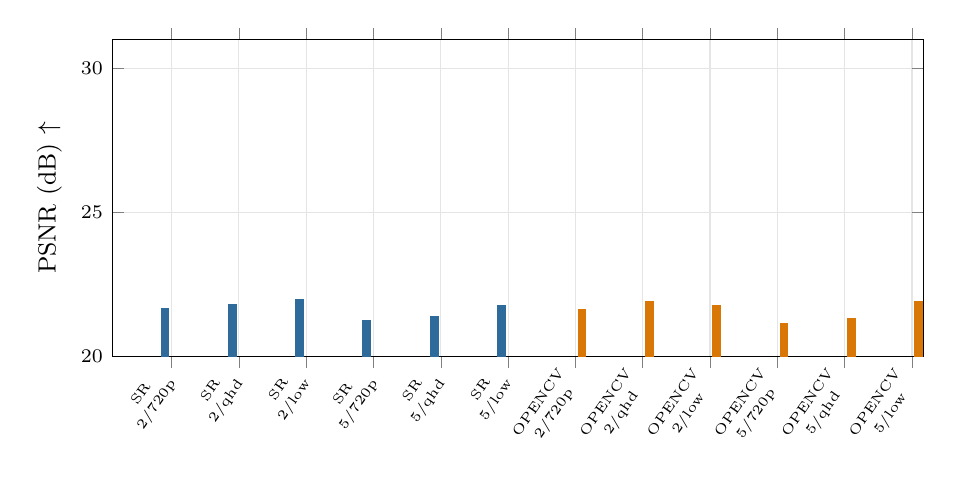
\begin{tikzpicture}
\begin{axis}[height=5.6cm,width=0.98\linewidth,ybar,bar width=2.8pt,enlarge x limits=0.015,xmin=-0.7,ymin=20,ymax=31,xtick=data,xticklabels={{\shortstack{SR\\2/720p}},{\shortstack{SR\\2/qhd}},{\shortstack{SR\\2/low}},{\shortstack{SR\\5/720p}},{\shortstack{SR\\5/qhd}},{\shortstack{SR\\5/low}},{\shortstack{OPENCV\\2/720p}},{\shortstack{OPENCV\\2/qhd}},{\shortstack{OPENCV\\2/low}},{\shortstack{OPENCV\\5/720p}},{\shortstack{OPENCV\\5/qhd}},{\shortstack{OPENCV\\5/low}}},x tick label style={font=\tiny,rotate=55,anchor=east},ylabel style={font=\small},tick label style={font=\scriptsize},ylabel={PSNR (dB) $\uparrow$},grid=major,grid style={gray!20},xtick={0,1,2,3,4,5,6,7,8,9,10,11}]
\addplot+[fill=srblue,draw=srblue,area legend] coordinates {(0,21.64427790) (1,21.78840496) (2,21.97335241) (3,21.22287166) (4,21.38360296) (5,21.77501791)};
\addplot+[fill=opencvorange,draw=opencvorange,area legend] coordinates {(6,21.63745354) (7,21.88344588) (8,21.76046466) (9,21.12845480) (10,21.30810001) (11,21.91248076)};
\end{axis}
\end{tikzpicture}
\par\vspace{2pt}
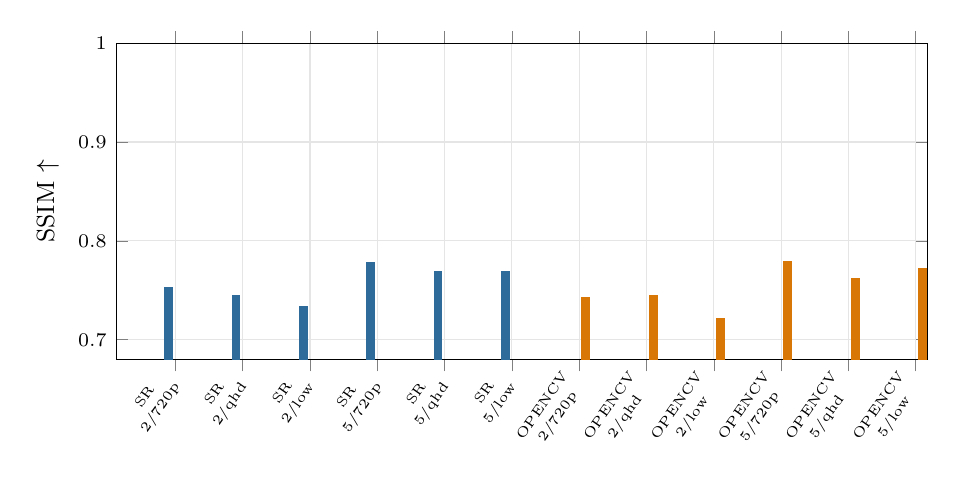
\begin{tikzpicture}
\begin{axis}[height=5.6cm,width=0.98\linewidth,ybar,bar width=2.8pt,enlarge x limits=0.015,xmin=-0.7,ymin=0.68,ymax=1.0,xtick=data,xticklabels={{\shortstack{SR\\2/720p}},{\shortstack{SR\\2/qhd}},{\shortstack{SR\\2/low}},{\shortstack{SR\\5/720p}},{\shortstack{SR\\5/qhd}},{\shortstack{SR\\5/low}},{\shortstack{OPENCV\\2/720p}},{\shortstack{OPENCV\\2/qhd}},{\shortstack{OPENCV\\2/low}},{\shortstack{OPENCV\\5/720p}},{\shortstack{OPENCV\\5/qhd}},{\shortstack{OPENCV\\5/low}}},x tick label style={font=\tiny,rotate=55,anchor=east},ylabel style={font=\small},tick label style={font=\scriptsize},ylabel={SSIM $\uparrow$},grid=major,grid style={gray!20},xtick={0,1,2,3,4,5,6,7,8,9,10,11}]
\addplot+[fill=srblue,draw=srblue,area legend] coordinates {(0,0.75282135) (1,0.74466826) (2,0.73409179) (3,0.77829448) (4,0.76856131) (5,0.76947999)};
\addplot+[fill=opencvorange,draw=opencvorange,area legend] coordinates {(6,0.74278970) (7,0.74503899) (8,0.72157909) (9,0.77870085) (10,0.76224984) (11,0.77217281)};
\end{axis}
\end{tikzpicture}
\par\vspace{2pt}
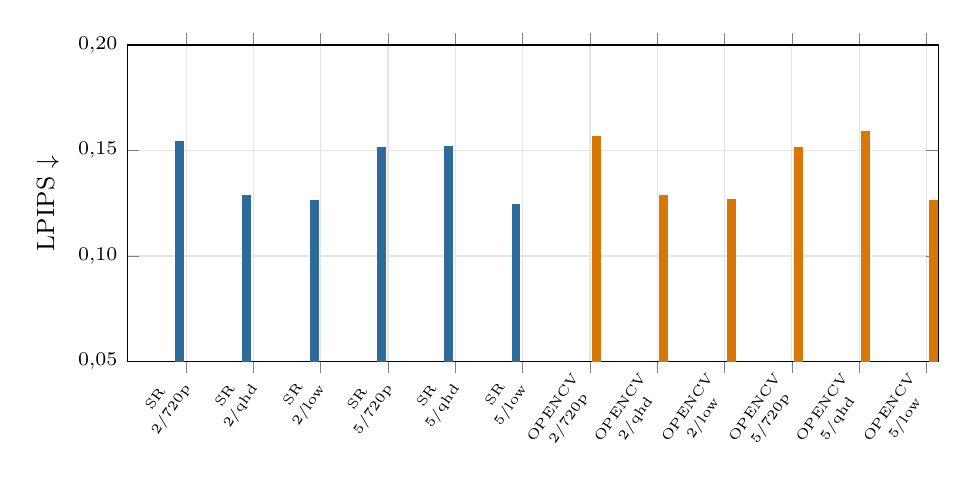
\begin{tikzpicture}
\begin{axis}[height=5.6cm,width=0.98\linewidth,ybar,bar width=2.8pt,enlarge x limits=0.015,xmin=-0.7,ymin=0.05,ymax=0.2,xtick=data,xticklabels={{\shortstack{SR\\2/720p}},{\shortstack{SR\\2/qhd}},{\shortstack{SR\\2/low}},{\shortstack{SR\\5/720p}},{\shortstack{SR\\5/qhd}},{\shortstack{SR\\5/low}},{\shortstack{OPENCV\\2/720p}},{\shortstack{OPENCV\\2/qhd}},{\shortstack{OPENCV\\2/low}},{\shortstack{OPENCV\\5/720p}},{\shortstack{OPENCV\\5/qhd}},{\shortstack{OPENCV\\5/low}}},x tick label style={font=\tiny,rotate=55,anchor=east},ylabel style={font=\small},tick label style={font=\scriptsize},ylabel={LPIPS $\downarrow$},grid=major,grid style={gray!20},scaled y ticks=false,ytick={0.05,0.10,0.15,0.20},yticklabels={{0,05},{0,10},{0,15},{0,20}},xtick={0,1,2,3,4,5,6,7,8,9,10,11}]
\addplot+[fill=srblue,draw=srblue,area legend] coordinates {(0,0.15446549) (1,0.12877836) (2,0.12619065) (3,0.15125681) (4,0.15200617) (5,0.12447236)};
\addplot+[fill=opencvorange,draw=opencvorange,area legend] coordinates {(6,0.15680037) (7,0.12855165) (8,0.12652283) (9,0.15150809) (10,0.15912115) (11,0.12632000)};
\end{axis}
\end{tikzpicture}
\par\vspace{2pt}
\vspace{3pt}
\begin{minipage}{0.98\linewidth}\scriptsize Alle zwölf Balkenpaare stammen aus \texttt{sugar\_coarse\_masked.json}; die STS-Baseline wird nicht als SuGaR-Ergebnis verwendet. PSNR/SSIM: höher ist besser; LPIPS: niedriger ist besser.\end{minipage}
\end{center}
\end{document}